\documentclass[10pt,leqno ]{article}

\usepackage{amsfonts}
\usepackage{amssymb}
\usepackage{array}
\usepackage{amsmath}
\usepackage{times}
\usepackage{mathtools}
\usepackage{amsthm}
\usepackage{hyperref}
\usepackage[margin=1.5in]{geometry}
\usepackage{setspace}
\usepackage{stmaryrd}
\usepackage{pgf}
\usepackage{tikz}
\usetikzlibrary{arrows,automata}

\DeclarePairedDelimiter\set\{\}

\newcommand\customeq[1]{\overset{\mathrm{#1}}{=}}
\newcommand\customarroweq[1]{\overset{\mathrm{#1}}{\Leftrightarrow}}

\newcolumntype{C}{>$c<$}


\newtheorem{theorem}{Theorem}
\theoremstyle{definition} 
\newtheorem{problem}[theorem]{Aufgabe}
     
\newenvironment{solution}[1][L]{\begin{doublespace}\textbf{#1.}\quad }{\ \rule{0.5em}{0.5em}\end{doublespace}}
    
\begin{document}

\begin{problem}
Mengengrundlagen
\end{problem}

\begin{solution}[a]
Gib die mit gelb gekennzeichnete Menge mit nur zwei Mengenoperationen an:

% Falsch wegen mehr als zwei Mengenoperationen (?)
\[ M = (A \setminus B) \triangle C \]

\end{solution}

\begin{solution}[b]
Berechne: \( (( \set{1,3} \times \set{1} )) \cup \set{1, 3, 1 } \setminus \set{(1,3), 1,2} \)

\begin{align*}
    M &= (( \set{1,3} \times \set{1} )) \cup \set{1, 3, 1 } \setminus \set{(1,3), 1,2} \\
    & \customeq{Def. \times} (\set{(1,1), (3,1)} \cup \set{1,3,1} \setminus \set{(1,3),1,2}) \\
    % hier fehlt vielleicht noch die reduktion von {1,3,1} zu  {1,3} (?)
    & \customeq{Def. \cup} (\set{(1,1),(3,1),1,3} \setminus \set{(1,3),1,2}) \\
    & \customeq{Def. \setminus} \set{(1,1),(3,1),3}
\end{align*}

\end{solution}

\begin{solution}[c]
Berechne: \( ( \set{\emptyset,2} \cup \set{\set{\emptyset}}) \cap \mathcal{P} (\set{ \set{\emptyset}, 2}) \)

\begin{align*}
    % Das P sieht eigentlich anders aus (?)
    M &= ( \set{\emptyset,2} \cup \set{\set{\emptyset}}) \cap \mathcal{P} (\set{ \set{\emptyset}, 2}) \\
    & \customeq{Def. \cup} \set{\emptyset, \set{\emptyset}, 2} \cap \mathcal{P} (\set{ \set{\emptyset}, 2}) \\
    & \customeq{Def. \mathcal{P}} \set{\emptyset, \set{\emptyset}, 2} \cap \set{\emptyset, \set{\set{\emptyset}}, \set{2}, \set{\set{\emptyset}, 2}} \\
    & \customeq{Def. \cap} \set{\emptyset}
\end{align*}

\end{solution}

\begin{problem}
Mengenbeweise
\end{problem}

\begin{solution}[a]
Beweise oder widerlege: Für alle Mengen A und B gilt: \( (A \cap B) \cap A = B \cap A \)

Wir beweisen die Aussage. Seien A, B beliebige Mengen.
\begin{align*}
    & & (A \cap B) \cap A = B \cap A \\
    & \customeq{Def. \cap} & \set{x \mid x \in \set{y \mid y \in A \land y \in B} \land x \in A} \\
    & \customeq{Komm.} & \set{x \mid x \in \set{y \mid y \in B \land y \in A} \land x \in A} \\
    & \customeq{Def. \in} & \set{x \mid (x \in B \land x \in A) \land x \in A} \\
    & \customeq{Assoz.} & \set{x \mid x \in B \land (x \in A \land x \in A)} \\
    & \customeq{Idem.} & \set{x \mid x \in B \land x \in A} \\
    & \customeq{Def. \cap} & B \cap A \\
\end{align*}

Somit gilt die Aussage.

\end{solution}

\begin{solution}[b]
Beweise oder widerlege: Für alle Mengen A und B gilt: \( A \cup (A \setminus B ) = A  \)

Wir beweisen die Aussage. Seien A, B beliebige Mengen.
\begin{align*}
    & & A \cup (A \setminus B ) = A \\
    & \customeq{Def. \cup} & \set{x \mid x \in A \lor x \in (A \setminus B)} \\
    & \customeq{Def. \setminus} & \set{x \mid x \in A \lor x \in \set{y \mid y \in A \land y \notin B}} \\
    & \customeq{Def. \in} & \set{x \mid x \in A \lor (x \in A \land x \notin B)} \\
    & \customeq{Distri.} & \set{x \mid (x \in A \lor x \in B) \land (x \in A \land x \in A)} \\
    & \customeq{Idem. oder} & \set{x \mid (x \in A \lor x \in B) \land x \in A} \\
    & \customeq{Absorp.} & \set{x \mid x \in A} \\
    & \customeq{Def. \in} & A \\
\end{align*}

Somit gilt die Aussage.

\end{solution}

\begin{solution}[c]
Beweise oder widerlege: Für alle Mengen A und B gilt: \( (B \cup A) \cap B = A \cap B \)

Wir widerlegen die Aussage durch Angabe eines geeigneten Gegenbeispiels.

Wir wählen \( A \triangleq \set{1,2}, B \triangleq \set{2,3} \).

\begin{align*}
    & & (B \cup A) \cap B  \\
    &= & (\set{2,3} \cup \set{1,2}) \cap \set{2,3}  \\
    & \customeq{Def. \cup} & \set{1,2,3} \cap \set{2,3}  \\
    &= & \set{2,3} \\
    & \neq & \set{2}  \\
    & \customeq{Def. \cap} & \set{1,2} \cap \set{2,3}  \\
    &= & A \cap B \\
\end{align*}

Somit gilt die Aussage nicht.

\end{solution}

\begin{problem}
    Wahrheitstabellen
\end{problem}

\begin{solution}[a]
Beweise oder widerlege nur mit Hilfe einer Wahrheitstabelle oder eines (Gegen-) Beispiels, dass \( \lnot q \land ((r \leftrightarrow (r \rightarrow \bot)) \lor q ) \) kontradiktorisch ist.

\[
\begin{array}{C|C||C|C|C|C|C|C|C|C|C|C}
q & r & $\lnot$ & q & $\overbrace{\land}^{\textbf{\(\downarrow\)}}$ & ((r & $\leftrightarrow$ & (r & $\rightarrow$ & $\bot$)) & $\lor$ & q) \\
\hline
F & F & W & F & F & F & F & F & W & F & F & F \\
F & W & W & F & F & W & F & W & F & F & F & F \\
W & F & F & W & F & F & F & F & W & F & W & W \\
W & W & F & W & F & W & F & W & F & F & W & W \\
\end{array}
\]

Der Hauptjunktor wird immer zu F ausgewertet. Also ist die Formel kontradiktorisch.


\end{solution}

\begin{solution}[b]
Beweise oder widerlege nur mit Hilfe einer Wahrheitstabelle oder eines (Gegen-) Beispiels, dass \( ((s \land \lnot q) \rightarrow r) \lor r \equiv r \lor (s \rightarrow q) \).


\[
\begin{array}{C|C|C||C|C|C|C|C|C|C|C||C|C|C|C|C}
q & r & s & ((s & $\land$ & $\lnot$ & q) & $\rightarrow$ & r) &  $\overbrace{\lor}^{\textbf{\(\downarrow\)}}$ & r & r & $\overbrace{\lor}^{\textbf{\(\downarrow\)}}$ & (s & $\rightarrow$ & q) \\
\hline
F & F & F & F & F & W & F & W & F & W & F & F & W & F & W & F \\
F & F & W & W & W & W & F & F & F & F & F & F & F & W & F & F \\
F & W & F & F & F & W & F & W & W & W & W & W & W & F & W & F \\
F & W & W & W & W & W & F & W & W & W & W & W & W & W & F & F \\
W & F & F & F & F & F & W & W & F & W & F & F & W & F & W & W \\
W & F & W & W & F & F & W & W & F & W & F & F & W & W & W & W \\
W & W & F & F & F & F & W & W & W & W & W & W & W & F & W & W \\
W & W & W & W & F & F & W & W & W & W & W & W & W & W & W & W \\
\end{array}
\]

Die beiden Hauptjunktoren werden in jeder Zeile zum selben Wert ausgewertet.
Also sind die beiden Formeln äquivalent.

\end{solution}


\begin{problem}
    Logische Äquivalenz
\end{problem}

\begin{solution}[a]
Gib an: eine Formel, die logisch äquivalent zu \( \bot \) ist und nur  \( \lnot \) und \( \lor \) als Operatoren enthält. 

\( \lnot (q \lor \lnot q) \equiv \bot \)
    
\end{solution}
    
\begin{solution}[b]
Beweise nur mit Hilfe von Äquivalenzumformungen, dass \( q \land (r \rightarrow s) \) und \( \lnot(r \lor \lnot q) \lor (s \land q) \) logisch äquivalent sind.    

\begin{equation*}
    \begin{aligned}
    & & q \land (r \rightarrow s) \\
    & \customeq{Implikation} & q \land (\lnot r \lor s)  \\
    & \customeq{Distr. von \land \textrm{über} \lor} & (\lnot r \land q) \lor (s \land q) \\
    & \customeq{De Morgan II} & \lnot(r \lor \lnot q) \lor (s \land q) \\
    \end{aligned}
\end{equation*}

\end{solution}


\begin{problem}
    Variablenbelegungen
\end{problem}

\begin{solution}[a]
Beweise ausschließlich mit Hilfe von Argumenten über eine oder mehrere Variablenbelegungen, dass \( q \rightarrow \lnot (r \land s) \equiv \lnot q \lor (r \rightarrow \lnot s) \).

\begin{equation*}
    \begin{aligned}
    & & \llbracket q \rightarrow \lnot (r \land s) \rrbracket ^ \beta = W \\
    & \customarroweq{Def. \rightarrow} & \llbracket q \rrbracket ^ \beta = F oder \llbracket \lnot (r \land s) \rrbracket ^ \beta = W  \\
    & \customarroweq{Def. De Morgan I} & \llbracket q \rrbracket ^ \beta = F oder \llbracket \lnot r \lor \lnot s \rrbracket ^ \beta = W  \\
    & \customarroweq{Def. Impl.} & \llbracket q \rrbracket ^ \beta = F oder \llbracket r \rightarrow \lnot s \rrbracket ^ \beta = W  \\
    & \customarroweq{Def. \lnot} & \llbracket \lnot q \rrbracket ^ \beta = W oder \llbracket r \rightarrow \lnot s \rrbracket ^ \beta = W  \\
    & \customarroweq{Def. \lor} & \llbracket \lnot q \lor r \rightarrow \lnot s \rrbracket ^ \beta = W  \\
    \end{aligned}
\end{equation*}

Damit wird \( q \rightarrow \lnot (r \land s) \) genau dann zu W ausgewertet, wenn \( \lnot q \lor (r \rightarrow \lnot s) \) zu W ausgewertet wird.
Also sind die beiden Formeln äquivalent.

\end{solution}
    
\begin{solution}[b]
Beweise oder widerlege ausschließlich mit Hilfe von Argumenten über eine oder mehrere Variablenbelegungen, dass \( \lnot (\lnot q \lor (s \land r)) \lor (q \leftrightarrow (s \land r)) \) allgemeingültig ist.

Betrachte die Belegung \( \beta \) mit \( \beta (q) = F \) und \( \beta (r) = \beta (s) = W \). Dann ist
\[ \llbracket \lnot (\lnot q \lor (s \land r)) \lor (q \leftrightarrow (s \land r)) \rrbracket = F \]

Damit ist die Formel nicht allgemeingültig (da es eine Belegung gibt, unter der die Formel zu F ausgewertet wird).

\end{solution}
    
\begin{problem}
    Prädikatenlogik
\end{problem}

\begin{solution}
Beweise: \( ((\exists y . P_1(y) \rightarrow P_2(y)) \land (\forall x . P_1(x))) \rightarrow \exists z . P_2(z) \land P_1(z) \)

Annahme (A1): \( ((\exists y . P_1(y) \rightarrow P_2(y)) \land (\forall x . P_1(x))) \)

Zu Zeigen (Z1): \( \exists z . P_2(z) \land P_1(z) \)

Annahme (A2): \( \exists y . P_1(y) \rightarrow P_2(y) \)

Annahme (A3): \( \forall x . P_1(x) \)

Wähle \(  x \triangleq y \) in A3

Annahme (A4): \( P_1(y) \)

Sei x (beliebig aber fest) in A2

Annahme (A5): \( P_1(y) \rightarrow P_2(y) \)

Aus A4 und A5 folgt A6

Annahme (A6): \( P_2(y) \)

Wähle \( z \triangleq y \) in Z1

Zu Zeigen (Z2): \( P_2(y) \land P_1(y) \)

Teil 1: Zu Zeigen (Z1.1): \( P_2(y) \)

\qquad Aus A6 folgt Z1.1

Teil 2: Zu Zeigen (Z2.1): \( P_1(y) \)

\qquad Aus A4 folgt Z2.1

\end{solution}

\begin{problem}
    Widerspruch und Kontraposition
\end{problem}

\begin{solution}[a]
    Ziehe, durch die schrittweise Anwendung logischer Äquivalenzen, alle Negationen inder folgenden Formel soweit wie möglich nach Innen. Begründe jeden Schritt.

    \begin{equation*}
        \begin{aligned}
        && \lnot(\lnot(\exists x . P_1(x)) \rightarrow (\forall y . P_2(y) \land P_3(y))) \\
        & \customeq{Def. Impl.} & \lnot(\lnot \lnot(\exists x . P_1(x)) \lor (\forall y . P_2(y) \land P_3(y))) \\
        & \customeq{Def. dopp. Neg.} & \lnot((\exists x . P_1(x)) \lor (\forall y . P_2(y) \land P_3(y))) \\
        & \customeq{Def.DeMorgan2} & \lnot(\exists x . P_1(x)) \land \lnot (\forall y . P_2(y) \land P_3(y)) \\
        & \customeq{Def. log.\textrm{Äquivalenz}} & (\forall x . \lnot P_1(x)) \land \lnot (\forall y . P_2(y) \land P_3(y)) \\
        & \customeq{Def. DeMorgan1} & (\forall x . \lnot P_1(x)) \land (\lnot(\forall y . P_2(y)) \lor \lnot P_3(y)) \\
        & \customeq{Def. log.\textrm{Äquivalenz}} & (\forall x . \lnot P_1(x)) \land (\exists y . \lnot P_2(y) \lor \lnot P_3(y)) \\
        \end{aligned}
    \end{equation*}
\end{solution}

\begin{solution}[b]
    Gib an: Den ersten Schritt, d.h. die erste Zeile, eines Beweises per Widerspruch für die
    Aussage \( \lnot(\exists x . P_1(x)) \rightarrow (\forall y . P_2(y) \land P_3(y)) \).

    Widerspruchs Annahme: 
    
    \( \lnot(\exists x . P_1(x)) \rightarrow (\forall y . P_2(y) \land P_3(y)) \equiv \lnot(\lnot(\exists x . P_1(x)) \rightarrow (\forall y . P_2(y) \land P_3(y))) \rightarrow \bot \)

\end{solution}

\begin{solution}[c]
    Gib an: Den ersten Schritt, d.h. die erste Zeile, eines Beweises per Kontraposition für die
    Aussage \( \lnot(\exists x . P_1(c)) \rightarrow (\forall y . P_2(y) \land P_3(y)) \).

    Zu Zeigen: \( \lnot(\forall y . P_2(y) \land P_3(y)) \rightarrow \lnot \lnot(\exists x . P_1(x))\)

\end{solution}

\begin{problem}
    Induktion
\end{problem}

\begin{solution}
    Beweise per Induktion \( \forall n \in \mathbb N_7 . n \bmod 2 = 1\).

    Hinweis H1: \( (n+m) \bmod r = ((n \bmod r)(m \bmod r)) \bmod r \)

    Sei  
    \begin{equation*}
        \begin{aligned}
        &  P(n) \triangleq (n\bmod 2 = 1 ) \\
        \end{aligned}
    \end{equation*}

    Wir verwenden das Induktionsschema: 
    \begin{equation*}
        \begin{aligned}
        & (P(7) \land (\forall n \land \mathbb N_7 . P(n) \rightarrow P(n+10)) ) \rightarrow (\forall x \in \mathbb N_7 . P(x)) \\
        \end{aligned}
    \end{equation*}

    \textbf{IA (}\(P(7)\)\textbf{)}:
    \begin{equation*}
        \begin{aligned}
        & 7\bmod 2 = 1 \\
        \end{aligned}
    \end{equation*}

    Sei \( n \in \mathbb N_7 \).

    \textbf{IV (}\(P(n)\)\textbf{)}:
    \begin{equation*}
        \begin{aligned}
        &  n \bmod 2 = 1 \\
        \end{aligned}
    \end{equation*}

    \textbf{IS (}\(P(n+10)\)\textbf{)}: Zu Zeigen: \( (n + 10) \bmod 2=1 \)
    \begin{equation*}
        \begin{aligned}
         (n + 10) \mod 2 \customeq{H1} & ((n \mod 2)+(10 \mod 2)) \mod 2 \\
        = & ((n \mod 2) + 0) \mod 2 \\
        \customeq{IV} & (1 + 0) \mod 2 \\
        = & 1 \mod 2 \\
        = & 1
        \end{aligned}
    \end{equation*}

    Nach unserem Induktionsschema gilt nun \( \forall x \in \mathbb N_7 . P(x) \) was äquivalent zur ursprünglichen Aussage ist. Damit ist die Aussage bewiesen.


\end{solution}

%%%%%%%%%%%%%%%%%%%%%%%%% HAUSAUFGABE 2 %%%%%%%%%%%%%%%%%%%%%%%
\pagebreak

\begin{problem}
    Eigenschaften von Relationen
\end{problem}

\begin{solution}[a]
   Gib die Relation \(R_4, R_5\) und \(R_6\) jeweils in Megenschreibweise an.
   
   $R_4$ \( \triangleq \set{ (b,2),(b,3),(c,2),(c,3),(c,1)} \)
   
   $R_5$ \( \triangleq \set{ (1,a),(2,a)} \)
   
   $R_6$ \( \triangleq \set{(a,b),(b,a),(c,b),(b,c)} \)
   
   
\end{solution}
\begin{solution}[b]
   Gib die Relation \(R_4, R_5\) und \(R_6\) jeweils graphisch an.
   
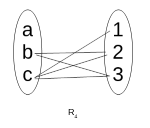
\includegraphics{abb/R4}
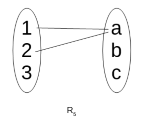
\includegraphics{abb/R5}
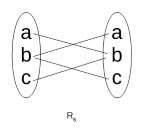
\includegraphics{abb/R6}

\end{solution}
\begin{solution}[c]
   Gib für jede der Relationen \(R_4\), \(R_5\) und \(R_6\) an, welche der Eigenschaften links-/rechtstotal
   und links-/rechtseindeutig erfüllt bzw. nicht erfüllt sind
   
   \begin{tabular}{|p{1cm}|p{3cm}|p{3cm}|p{3cm}|p{3cm}|}
     \hline
        & linkstotal & rechtstotal& linkseindeutig& rechtseindeutig\\    
     \hline
       $R_4$  & X &  \(\surd \) & X & X  \\
     \hline
       $R_5$ & X  & X & X&  \(\surd \) \\
     \hline
       $R_6$ & \(\surd \) &  \(\surd \) & X & X \\
     \hline
   \end{tabular}
   
\end{solution}
\begin{solution}[d] 
Gib zwei Mengen X, Y so an, dass jede rechtstotale, rechtseindeutige Relation R : (X, Y)
linkseindeutig ist.
   
   Wenn 
   X= \(\set {\emptyset} \)
   und Y= \(\set {\emptyset}\)
   ist jede Relation R:(X,Y), die rechtstotal und rechtseindeutig ist, linkseindeutig, da die leere Relation \(\emptyset_{X,Y}\) immer linkseindeutig ist.

   
\end{solution}

\begin{problem}
Homogene Relation
\end{problem}

   \( C \triangleq \set{ a,b,c,d} \)

   $R_7$(C,C) mit $R_7$= \( \set{ (a,a),(a,c),(c,b),(d,c),(d,d)} \)

\begin{solution}[a]
Berechne t(\(R_7\)) schrittweise.

\begin{equation*}
   \begin{aligned}
    & R_{7}^1 \customeq{FS 2.1.16} R_7 \\
    & R_{7}^2 \customeq{FS 2.1.16} R_{7}R_{7} \customeq{Def. ;} \set{(a,b),(d,b)}\\
    & R_{7}^3 \customeq{FS 2.1.16} R_{7}R_7^2 \customeq{Def. ;} \emptyset\\
    & R_{7}^4 \customeq{FS 2.1.16} R_{7}R_7^3 \customeq{Def. ;} R_7^3 \\
    & t(R_7) \customeq{Def. t(\cdot)} \bigcup\limits_{n \in N^+} R_7^n = R_7 \cup R_7^2 \cup R_7^3\\
    & \customeq{Def. \cup} \set{(a,a),(a,b),(a,c),(c,b),(d,b),(d,c),(d,d)}
   \end{aligned}
\end{equation*}

\end{solution}

\begin{solution}[b]
Gib für $R_8$ \( \triangleq t(R_7) \cup \Delta_C \) an, welche der Ordnungsbegriffe Quasiordnung, partielle Ordnung und totale Ordnung erfüllt bzw. nicht erfüllt sind.

\( \Delta_C = \set{(a,a),(b,b),(c,c),(d,d)} \)

$R_8$ = \( \Delta_C \cup t(R_7)\customeq{Def. \cup} \set{(a,a),(a,b),(a,c),(b,b),(c,b),(c,c),(d,b),(d,c),(d,d)} \)

\begin{equation*}
   \begin{aligned}
   reflexiv: \\
   &\Delta_C \customeq{Def. \Delta} \set{(a,a),(b,b),(c,c),(d,d)} \subseteq{}R_8\\
   transitiv:\\ 
   & R_8R_8 \customeq{Def. ;} R_8\subseteq R_8\\
   antisymmetrisch:\\
   & R_8^{-1} \cap R_8 \customeq{Def. ^{-1}} \set{(a,a),(b,a),(b,b),(c,a),(b,c),(c,c),(b,d),(c,d),(d,d)} \cap R_8\\
   &\customeq{Def. \cap} \set{(a,a),(b,b),(c,c),(d,d)} \customeq{Def. \Delta} \Delta_C \subseteq{}R_8\\
   linear:\\
   &\nabla_{C,C} \setminus \Delta_C\\
   &\customeq{Def. \Delta} \nabla_{C,C} \setminus \set{(a,a),(b,b),(c,c),(d,d)}\\
   &\customeq{Def. \nabla} \set{(a,a),(a,b),(a,c),(a,d),(b,a),(b,b),(b,c),(b,d),(c,a),(c,b),(c,c),\\&(c,d),(d,a),(d,b),(d,c),(d,d)} \setminus \set{(a,a),(b,b),(c,c),(d,d)}\\
   &\customeq{Def. \setminus} \set{(a, b),(a, c),(a, d),(b, a),(b, c),(b, d),(c, a),(c, b),(c, d),(d, a),(d, b),(d, c)}\\
   &\customeq{Def. \subseteq}\nabla_{C,C} \setminus \Delta_C \not \subseteq R_8\\
    \end{aligned}
\end{equation*}

\(R_8\) ist reflexiv, transitiv, antisymmetrisch und nicht linear, da $(a,d)$ nicht enthalten in $R_8$, und somit ist $R_8$ eine quasi Ordnung, eine partielle Ordnung, aber keine totale Ordnung.
\end{solution}

\begin{solution}[c]
Sei $R_9 :(C,C)$ mit $R_9 \triangleq \set{ (a, a), (a, b), (b, b), (c, c), (c, d), (d, d) }$\\
\begin{equation*}
    \begin{aligned}
    reflexiv:\\ 
    &\Delta_C \customeq{Def. \Delta} \set{(a,a),(b,b),(c,c),(d,d)} \subseteq{}R_8\\
    transitiv:\\ 
    & R_8R_8 \customeq{Def. ;} R_8\subseteq R_8\\
    antisymmetrisch:\\
    & R_8^{-1} \cap R_8 \customeq{Def. ^{-1}} \set{(a,a),(b,a),(b,b),(c,c),(d,c),(d,d)} \cap R_8\\
    &\customeq{Def. \cap} \set{(a,a),(b,b),(c,c),(d,d)} \customeq{Def. \Delta} \Delta_C \subseteq{}R_8\\
    \end{aligned}
\end{equation*}
   $R_9$ ist reflexiv, transitiv und antisymmetrisch und somit eine partielle Ordnung. \\
\end{solution}

\begin{solution}[d]
    Beweise: $R_9$ ist keine totale Ordnung.
\begin{equation*}
    \begin{aligned}
    linear:\\
    \nabla_{C,C} \setminus \Delta_C\\
    \customeq{Def. \Delta} \nabla_{C,C} \setminus \set{(a,a),(b,b),(c,c),(d,d)}\\
    \customeq{Def. \nabla} \set{(a,a),(a,b),(a,c),(a,d),(b,a),(b,b),(b,c),(b,d),(c,a),(c,b),(c,c),\\
    (c,d),(d,a),(d,b),(d,c),(d,d)} \setminus \set{(a,a),(b,b),(c,c),(d,d)}\\
    \customeq{Def. \setminus} \set{(a, b),(a, c),(a, d),(b, a),(b, c),(b, d),(c, a),(c, b),(c, d),(d, a),(d, b),(d, c)}\\
    \customeq{Def. \subseteq}\nabla_{C,C} \setminus \Delta_C \not \subseteq R_8\\
    \end{aligned}
\end{equation*}
Das Paar $(a,c)$ ist nicht enthalten und damit ist $R_9$ nicht linear und somit keine totale Ordnung. \\
\end{solution}
%%%%%%%%%%%%%%%%%

\begin{problem}
    Abbildungen, Funktionen
\end{problem}
\begin{solution}[a]

\textit{Gib an: Welche der Relationen \(R_1\), \(R_2\), \(R_3\) und \(R_4\) sind (keine) partiellen bzw. totalen Abbildungen?}

Die Relationen \(R_1\) und \(R_2\) sind keine partiellen bzw. totalen Abbildungen. 
Die Relation \(R_3\) ist eine partielle Abbildung und die Relation \(R_4\) ist eine totale Abbildung.

\textit{Gib an: Für jede der Relationen, die keine partielle Abbildung ist, ein Gegenbeispiel, dass das begründet.}

Die Relation \(R_1\) ist keine partielle Abbildung, weil die Paare \((d,b)\) und \((d,5)\) in der Relation auftreten.
Die Relation \(R_2\) ist keine partielle Abbildung, weil die Paare \((5,5)\) und \((5,d)\) in der Relation auftreten.
\end{solution}

\begin{solution}[b]

\textit{Gib an: Welche der Eigenschaften injektiv, surjektiv und bijektiv werden durch die Relationen \(R_1\), \(R_2\), \(R_3\) und \(R_4\) (die partielle oder totale Abbildungen sind) erfüllt / nicht erfüllt?}

\(R_3\) ist injektiv, surjektiv und bijektiv.

\(R_4\) ist weder injektiv, surjektiv noch bijektiv. 

\textit{Gib für jede nichterfüllte Eigenschaft ein Gegenbeispiel oder eine Begründung an.}

Die Abbildung \(R_4\) ist nicht injektiv, weil die Paare \((5,5)\) und \((d,5)\) in der Relation auftreten.
Die Abbildung \(R_4\) ist nicht surjektiv, weil das Element \(3\) aus dem Zielbereich \(A\) nicht mit einem anderen Element aus dem Argumentbereich \(B\) in Relation steht.
Die Abbildung \(R_4\) ist nicht bijektiv, weil sie nicht injektiv und nicht surjektiv ist.
\end{solution}

\begin{solution}[c]

\textit{Beweise oder widerlege: Für alle Funktionen \(f: B \rightarrow C, g: A \rightarrow B\) mit beliebigen Mengen A, B und C gilt, wenn \(f \circ g\) surjektiv ist, dann ist g surjektiv.}

Wir widerlegen die Aussage durch Angabe eines Gegenbeispiels.

Wir wählen die Mengen A, B und C mit: \(A \triangleq \set{1,2}\), \(B \triangleq \set{3,4}\), \(C \triangleq \set{5}\).

Wähle g: \(A \rightarrow B\) mit \(g \triangleq \set{(1,3)} \triangleq R_1\) und f: \(B \rightarrow C\) mit \(f \triangleq \set{3,5} \triangleq R_2\).

\((f \circ g) \customeq{Def. \circ} \set{(1,5)}\), wobei gilt, dass \(\forall c \in C . \exists a \in A . aR_2c\). Daraus folgt, dass \((f \circ g)\) surjektiv ist.

Für die gewählte Funktion g gilt aber nicht \(\forall b \in B . \exists a \in A . aR_1b\). Daraus folgt, dass g nicht surjektiv ist.

Somit ist die Aussage widerlegt.
\end{solution}

\begin{problem}
Kardinalität

Sei \(M \triangleq \set{n \in \mathbb{N} | n \bmod 10 = 7}\)

Beweise oder widerlege: \(card(M) = card(\mathbb{N})\)
\end{problem}
\begin{solution}
Wir beweisen die Aussage und geben eine Bijektion f: \(M \rightarrow \mathbb{N}\) an.
\begin{align*}
    f: M &\rightarrow \mathbb{N} \\
    x &\mapsto (x - 7) : 10 \\ 
\end{align*}

Die Funktion ist für jedes \(x \in M\) eindeutig definiert und bildet ausschließlich auf ganze Zahlen ab.

Wir geben eine weitere Funktion g: \(\mathbb{N} \rightarrow M\) an.
\begin{align*}
    f: \mathbb{N} &\rightarrow M \\
    x &\mapsto 10x + 7 \\ 
\end{align*}

Zu Zeigen (Z1): Bijektion(f)

Wenn \((f \circ g) = \Delta_\mathbb{N} \) und \((g \circ f) = \Delta_M \), dann ist laut Formelsammlung 2.2.8 f eine Bijektion.

Teil 1: Zu Zeigen (Z1.1): \(\forall x \in \mathbb{N} . (f \circ g)(x) = \Delta_\mathbb{N}(x) \)
Sei \(x \in \mathbb{N}\) beliebig aber fest.
\begin{equation*}
    \begin{aligned}
    && (f \circ g)(x) \\
    & \customeq{Def. \circ} & f(g(x)) \\
    & \customeq{Def. g} & f(10x + 7) \\
    & \customeq{Def. f} & ((10x + 7) - 7) : 10 \\
    & = & x \\
    & \customeq{Def. \Delta} & \Delta_\mathbb{N}(x) \\
    \end{aligned}
\end{equation*}

Teil 2: Zu Zeigen (Z2.1):  \(\forall x \in M . (g \circ f)(x) = \Delta_M(x) \)
Sei \(x \in M\) beliebig aber fest.
\begin{equation*}
    \begin{aligned}
    && (g \circ f)(x) \\
    & \customeq{Def. \circ} & g(f(x)) \\
    & \customeq{Def. f} & g((x - 7) : 10) \\
    & \customeq{Def. g} & 10*((x-7):10) + 7 \\
    & = & x \\
    & \customeq{Def. \Delta} & \Delta_M(x) \\
    \end{aligned}
\end{equation*}

Da wir Z1.1 und Z2.1 gezeigt haben, gilt: f ist eine Bijektion. Somit gilt die Aussage.
\end{solution}

\begin{problem}
    Äquivalenzen
\end{problem}
\begin{solution}[a]

    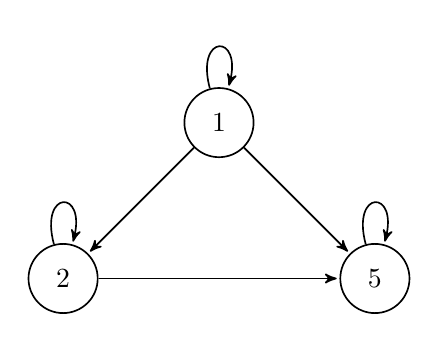
\begin{tikzpicture}[->,>=stealth',shorten >=1pt,auto,node distance=2.8cm,
        semithick]
    \tikzstyle{every state}=[fill=white,draw=black,text=black]
    
    \node[state] (1)                    {$1$};
    \node[state] (2) [below left of=1]  {$2$};
    \node[state] (5) [below right of=1] {$5$};
    
    \path   (1) edge node {} (2)
                edge [loop above] node {} (1)
                edge node {} (5)
            (2) edge node {} (5)
                edge [loop above] node {} (2)
            (5) edge [loop above] node {} (5);

                
    \end{tikzpicture}
    
    \begin{tikzpicture}[->,>=stealth',shorten >=1pt,auto,node distance=2.8cm,
        semithick]
    \tikzstyle{every state}=[fill=white,draw=black,text=black]
    
    \node[state] (3)                    {$3$};
    \node[state] (0) [right of=1]       {$0$};
    
    \path   (3) edge node {} (0)
                edge [loop above] node {} (3)
            (0) edge [loop above] node {} (0);
    \end{tikzpicture}
    
    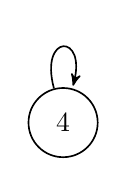
\begin{tikzpicture}[->,>=stealth',shorten >=1pt,auto,node distance=2.8cm,
        semithick]
    \tikzstyle{every state}=[fill=white,draw=black,text=black]
    
    \node[state] (4)                    {$4$};
    
    \path   (4) edge [loop above] node {} (4);
    \end{tikzpicture}

\end{solution}

\begin{solution}[b]

    A/$R_1$ hat 3 Äquivalenzklassen
    A/$R_1$ = \{ $[1]_{R_1}$, $[0]_{R_1}$, $[4]_{R_1}$ \}
    
    mit $[1]_{R_1}$ = \{1,2,5\}, $[0]_{R_1}$ = \{3,0\} und $[4]_{R_1}$ = \{4\} 

\end{solution}

\begin{solution}[c]
    Beweise: \( \forall x,y \in X. (x,y)\in R \rightarrow x=y \)

    Zu Zeigen (Z0):  \( \forall x,y \in X. (x,y)\in R \rightarrow x=y \)

    Sei x,y beliebig in X

    Zu Zeigen (Z1): \( (x,y) \in R \rightarrow x=y \)

    Annahme (A0) : \( (x,y) \in R \)

    Zu Zeigen (Z2): \( x=y \)
    
    Aus der Eigenschaft der Antisymmetrie und (A0) folgt

    (A1) \( \forall x,y \in X. xRy \land yRx \rightarrow x=y \)

    Aus (A0) und (A1) folgt

    (A2) \( x = y \)

\end{solution}


\begin{problem}
    Repräsentantensysteme
\end{problem}

\begin{solution}[a]

    \(R \triangleq \{ (a,b) | (a-b) \bmod 9 = 0 \} \)

\end{solution}

\begin{solution}[b]
    
    A/$R$ hat 3 Äquivalenzklassen
    A/$R$ = \{ $[2]_R$, $[5]_R$, $[8]_R$ \} mit 

    $[2]_R$ = \{ \( n \in \mathbb{N} | n \bmod 9 = 2 \) \}

    $[5]_R$ = \{ \( n \in \mathbb{N} | n \bmod 9 = 5 \) \}

    $[8]_R$ = \{ \( n \in \mathbb{N} | n \bmod 9 = 8 \) \}

\end{solution}

\begin{solution}[c] 

    \( P \triangleq \{ 2,5,8 \} \)
    
\end{solution}

\begin{solution}[d]

    \( f: \{ a,b,c \} \rightarrow P \) mit \(f \triangleq \{ (a,2), (b,5), (c,8) \}\)
    
\end{solution}

\begin{problem}
    Kern einer Abbildung
\end{problem}
\begin{solution}[a]
    
\( Ker(f) = \{ (a,c), (c,a), (a,e), (e,a), (c,e), (e,c), (d,f), (f,d), (a,a), (b,b), (c,c), (d,d), (e,e) \} \)

\end{solution}

\begin{solution}[b]

    \( f:D \rightarrow \mathbb{N} \) mit \( ((n \bmod 3) + 1) * 4 + 1 \)

\end{solution}

\begin{solution}[c]

    Antwort: \( card(X) > card(Y) \)
    
\end{solution}

\pagebreak

\begin{problem}
    Wörter und Sprachen
\end{problem}
Gegeben sei das Alphabet \(\lambda = \set{ a, b, c }\).\\
\\
\begin{solution}[a]Gib alle Präfixe der Wörter ac und bca an.

 \(\set{\lambda ,a ,c ,b ,bc ,bca}  \)\\

\end{solution}
\begin{solution}[b]Gib eine Menge von maximal 5 Wörtern über dem Alphabet \(\Sigma\) so an, dass die Suffixe
dieser Wörter genau aus den Wörtern\(\lambda\), a, b, c, ac, bb, cb, ccb bestehen\\
\(M =\set{a, bb , ac, ccb}\)\\

\end{solution}
\begin{solution}[c]Gib ein Wort über dem Alphabet \(\Sigma\) so an, dass die Anzahl der Teilwörter und die Summe
der Anzahl der Präfixe und Suffixe gleich 10 ist.\\

\( w= abca  \in \Sigma^* \)\\
\end{solution}
\pagebreak
\begin{problem}
Reguläre Ausdrücke
\end{problem}
Gegeben sei das Alphabet \(\Sigma = \set{ a, b, c }\).

\begin{solution}[a]Gib die Sprache L(\(e_1\)) für den regulären Ausdruck \(e1 , a0a + ac (b + e)^* + d + cc^*\) an,ohne auf reguläre Ausdrücke zu verweisen. \\
\(L(e_1)   \triangleq (w \in \Sigma^* \mid w \in {ac(b)^*,d,cc^*})\)


\end{solution}



\begin{solution}[b]
\(e_2 \triangleq ((b)^*a(b)^*a(b)^*a(b)^*)^+ + d + c^* + (c)^*d(c)^* + ((c)^*(d)^+(c)^*(d)^+(c)^*(d)^+(c)^*)^*\)


\end{solution}

\begin{problem}
Ordnen von Wörtern
\end{problem}
\begin{solution}[a]

\(\lambda \ll_{R1} 312 \ll_{R1} 32 \ll_{R1} 120 \ll_{R1} 032 \ll_{R1} 0 \ll_{R1} 02 \)


\end{solution}
\begin{solution}[b]

\( \lambda \ll_{R2}^S 23 \ll_{R2}^S 30 \ll_{R2}^S 231 \ll_{R2}^S 230 \ll_{R2}^S 000 \)



\end{solution}
\begin{solution}[c]

\( R_3 = t(r(\set{(2,0),(0,3),(3,1)})) \)


\end{solution}
\pagebreak
\begin{problem}
    Induktion über Wörter
\end{problem}

\begin{solution}
Beweise per (Wort)Induktion das \( \forall w \in \sum^* . bin(w) \geq \vert w \vert_1 \) \\

bin(w) kann nicht kleiner sein als \(\vert w \vert_1 \)da für jede 1 die in w enthalten ist mindestens 1 zum Wert von bin(w) hinzugefügt wird. Die Funktion w ändert von der letzten Stelle nach vorne und verdoppelt bei jedem Schritt den Multiplikator von der Binärstelle und startet bei 1. Dadurch muss jede 1 in w mindestens 1 zur Endzahl hinzuaddieren.\\
Bsp. w=10110 

\(\vert 10110 \vert_1 \) = 3\\
Bin(10110)= Bin(1011)+1*0\\
Bin(1011)=Bin(101)+2*1+1*0\\
Bin(101)=Bin(10)+4*1+2*1+1*0\\
Bin(10)=Bin(1)+8*0+4*1+2*1+1*0\\
Bin(1)=Bin(\(\lambda\))+16*1+8*0+4*1+2*1+1*0\\
Bin(\(\lambda\))=0+16*1+8*0+4*1+2*1+1*0=22\\
$22\geq 3$


\end{solution}

\begin{problem}
    Grammatiken und Sprachen
\end{problem}

\begin{solution}[a]

    \(S \Rightarrow_{G_1} bV \Rightarrow_{G_1} bcbS \Rightarrow_{G_1} bcbaaU \Rightarrow_{G_1} bcbaacU \Rightarrow_{G_1} bcbaacc \)

\end{solution}

\begin{solution}[b]

    \( L(G_1) = \{ x^{n}y \mid n \in \mathbb{N} \text{ mit } x = \{bca^{m}b \mid m \in \{0,1\}\} \text{ und } y = \{aavc \mid v \in \{b,c\}^{*}\} \} \)

\end{solution}

\begin{solution}[c]

    \(S \Rightarrow_{G_2} cT \Rightarrow_{G_2} cbbTaa \Rightarrow_{G_2} cbbabTaaa \Rightarrow_{G_2} cbbabcaaa \)
    
\end{solution}

\begin{solution}[d]

    \( L(G_2) = \{ cb^{2n}(ab)^{m}b^{2o}c(aa)^{n+o}a^{m} \mid n,m,o \in \mathbb{N} \} \)

    % oder

    % \( L(G_2) = \{ c(bb)^{n}(ab)^{m}(bb)^{o}ca^{2+(n+o)+m} \mid n,m,o \in \mathbb{N} \} \)
    
\end{solution}

\begin{problem}
    Sprachen und Grammatiken
\end{problem}

\begin{solution}[a]

    \( G_3 = ( \{ S,T,U \}, \sum, P_3, S ) \) mit 

    $P_3:$ 

    \( S \to cT \)

    \( T \to aU \mid bU \mid a \mid b \)

    \( U \to aaU \mid bbU \mid abU \mid baU \)

\end{solution}

\begin{solution}[b]

    \( G_4 = ( \{ S,T,U \}, \sum, P_4, S ) \) mit 

    $P_4:$ 

    \( S \to bbT \) 

    \( T \to bTc \mid bTac \mid aU \) 

    \( U \to aU \mid cc \) 
    
\end{solution}

\begin{problem}
    Chomsky Hierarchie
\end{problem}

\begin{solution}[a]
    
    \( G_1 \to \text{ Typ 2 Grammatik}\)

    \( G_2 \to \text{ Typ 1 Grammatik}\)

\end{solution}

\begin{solution}[b]

    \( A_3 \to \text{ ist regulär (Typ 3)} \)

    \( A_4 \to \text{ ist kontextfrei (Typ 2)} \)
    
\end{solution}

\begin{solution}[c]

    \( G_5 = ( \{ S,T,U,V,W \}, \{ a,b \}, P_5, S ) \) mit 

    $P_5:$ 

    \( S \to aT \mid cU \) 

    \( T \to aT \mid cW \mid c \) 

    \( U \to bV \mid b \)

    \( V \to bU \)

    \( W \to bW \mid b \)

    
\end{solution}

\begin{problem}
    Reguläre Sprachen / Pumping Lemma
\end{problem}

\begin{solution}[a]

    Seien $m \in \mathbb{N}$ beliebig und fest. Wir wählen das Wort $w = a^{m}c^{m}b^{m+7}$ mit $w 
    \in A_1$ und $|w| \geq m$. Sei $w=xyz$ eine beliebige Zerlegung mit $y \neq \lambda$ und $|xy| \leq m $. Dann ist $x=a^{i}$, $y=a^{j}$, $z=a^{m-i-j}c^{m}b^{m+7}$ für $j \neq 0$ und $i+j \leq m$. Wir wählen $k=0$. Dann ist $xy^{0}z=a^{m-j}c^{m}b^{m+7}$, somit ist $xy^{0}z \notin A_1 $, denn der Abstand von $m-j$ zu $m+7$ kann nicht mehr 7 betragen, da $j \neq 0$ ist.
    
\end{solution}

\begin{solution}[b]

    Sei $m \in \mathbb{N} w = cb^{m-3}ca^{m}$ mit $w \in A_2$, denn $cb^{m-3}ca^{m} = cxca^{m}$ für $x \in {c,b}^{*}$ und $ |cb^{m-3}c < m$ und $|w| \geq m$

    Sei $w=xyz$ eine beliebige Zerlegung mit $y \neq \lambda$ und $|xy| \leq m $

    1.Fall: $x=cb^{i}$, $y=b^{j}c$, $z=a^{m}$ für $i+j = m-3$. Wir wählen $k=0$. Dann ist $xy^{0}z = cb^{i}a^{m}$. $cb^{i}a^{m}\notin A_2$ 

    2.Fall: $x=cb^{m-3}$, $y=c$, $z=a^{m}$. Wir wählen $k=0$. Dann ist $xy^{0}z = cb^{m-3}a^{m}$. $cb^{m-3}a^{m} \notin A_2$ 

    3.Fall: $x=c$, $y=b^{m=3}c$, $z=a^{m}$. Wir wählen $k=0$. Dann ist $xy^{0}z = ca^{m}$. $ca^{m} \notin A_2$ 

    4.Fall: $x=\lambda$, $y=cb^{m-3}c$, $z=a^{m}$. Wir wählen $k=0$. Dann ist $xy^{0}z = a^{m}$. $a^{m} \notin A_2$ 
    
\end{solution}



\begin{problem}
    DFA
\end{problem}

\begin{solution}[a]

    \( (q_1,bb) \vdash (q_2,b) \vdash (q_3,\lambda) \not \vdash \)

    da $q_3$ $\notin \{ q_2 \}$, ist bb $\notin L(M_3)$  

    \( (q_1,ccbc) \vdash (q_0,cbc) \vdash (q_1,bc) \vdash (q_2,c) \vdash (q_2,\lambda) \not \vdash \)
    
    da $q_2$ $\in \{ q_2 \}$, ist ccbc $\in L(M_3)$ 
    
\end{solution}

\begin{solution}[b]
    
    \( (q_0,abc) \vdash (q_1,bc) \vdash (q_1,c) \vdash (q_2,\lambda)  \not \vdash \)
    
    da $q_2$ $\in \{ q_0,q_2 \}$, ist abc $\in L(M_4)$

    \( (q_0,cbc) \vdash (q_2,bc) \vdash (q_2,c) \vdash (q_1,\lambda) \not \vdash \)
    
    da $q_1$ $\notin \{ q_0,q_2 \}$, ist cbc $\notin L(M_4)$
    
\end{solution}

\begin{solution}[c]

    \( L(M_3) = \{ w \in c^{n}bc^{m} \mid n,m \in \mathbb{N} \text{ und } |w| > 0 \} \)
    
\end{solution}

\begin{solution}[d]

    \( L(M_4) = \{ w \in \{ a,b,c \}^{*} \mid (\exists x \in \{ b,c \}. \exists n \in \{ 0,1 \}, m \in \mathbb{N}. w = a^{n}x^{m} \land |w|_C \mod 2 = 1) \lor |w|=0 \} \)
    
\end{solution}

\begin{problem}
    Automat zu einer Sprache
\end{problem}

\begin{solution}[a]

    $\delta_{5}$:


        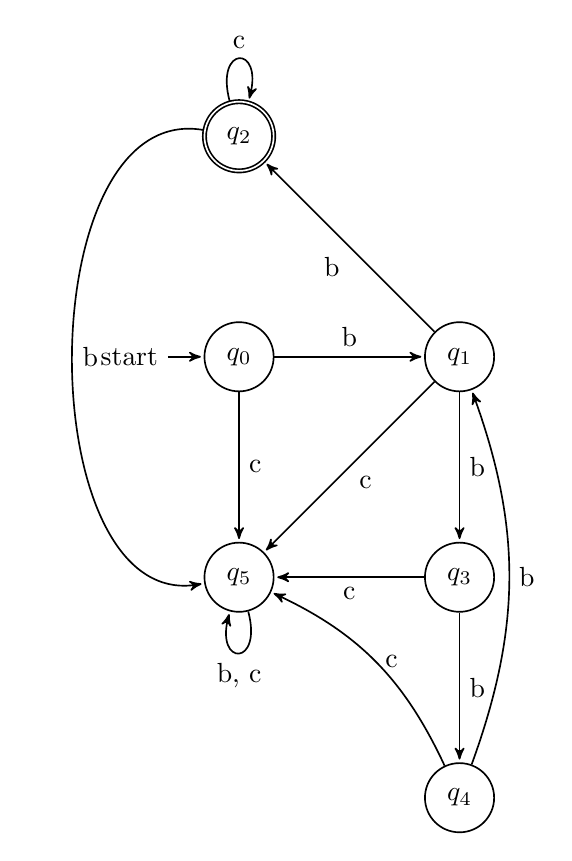
\begin{tikzpicture}[->,>=stealth',shorten >=1pt,auto,node distance=2.8cm,
            semithick]
        \tikzstyle{every state}=[fill=white,draw=black,text=black]
        
        \node[initial,state] (0) {$q_0$};
        \node[state] (1) [right of=0] {$q_1$};
        \node[state, accepting] (2) [above of=0] {$q_2$};
        \node[state] (3) [below of=1] {$q_3$};
        \node[state] (4) [below of=3] {$q_4$};
        \node[state] (5) [below of=0] {$q_5$};
        
        \path
            (0) edge node {b} (1)
                edge node {c} (5)
            (1) edge node {b} (2)
                edge node {b} (3)
                edge node {c} (5)
            (2) edge [loop above] node {c} (2)
                edge [right , bend right =100] node {b} (5)
            (3) edge node {b} (4)
                edge node {c} (5)
            (4) edge [right , bend right =20] node {b} (1)
                edge [right , bend right =20] node {c} (5)
            (5) edge [loop below] node {b, c} (5);

        \end{tikzpicture}
    
\end{solution}


\end{document}